% Artificial Intelligence Lab Report -- compile with pdfLaTeX and BibTeX
%   pdflatex main && bibtex main && pdflatex main && pdflatex main
\documentclass{ai-lab-report}

% ---------- Student details ----------
\title{Search, Constraint Satisfaction, Swarms and Sequential Decisions:\\
       Four AI Methods on Four Dhaka Problems}
\reportemail{kabyasaha1812@gmail.com}
\author{Kabya Mithun Saha}
\date{\today}

\begin{document}
\maketitle

\begin{abstract}
This report covers three Artificial Intelligence laboratory assignments, the third of
which has two parts. In Assignment~1 we route a traveller across the real
OpenStreetMap road graph of Dhaka (28{,}094 intersections, 70{,}197 segments) under a
twelve-factor cost model, and compare three uninformed and three informed search
algorithms against six heuristics. In Assignment~2 we model a citywide fuel shortage as
a constraint optimisation problem and compare five solvers, including forward checking
with MRV and a min-conflicts local search. Assignment~3 asks for a problem that a single
weak agent cannot solve but a population can. Part~A places Wi-Fi access points on a
university hall floor with a particle swarm optimiser written from scratch; the key
result is an ablation showing that thirty particles which do not communicate are
statistically no better than random search, while the same thirty sharing a single number
gain 2.47 points of coverage. Part~B models the hall's water tank under Dhaka load-shedding as a Markov
decision process and compares Value Iteration (model-based) against Q-learning
(model-free). Our main finding there is negative and, we think, the more useful
one: a roughly-right model is worth more than 82 simulated years of experience, and even a
fourfold error in the model still beats Q-learning. Model-free learning earns its place only
when the transition structure cannot be written down at all.
\end{abstract}

\keywords{Artificial Intelligence; heuristic search; constraint satisfaction; particle
swarm optimisation; Markov decision processes; reinforcement learning}
\vspace{5mm}
% NOTE: the supplied template has a bare \hline here, which is a LaTeX error
% outside a tabular ("Misplaced \noalign") and stops the build. A rule does the
% same job and compiles.
\noindent\rule{\textwidth}{0.4pt}

\section{Introduction}
All four problems in this report are set in Dhaka. That is deliberate. Each
assignment asks for a different class of AI method, and the easiest way to understand
why a method exists is to point it at a problem it was built for and then at one it was
not.

Assignment~1 is a search problem: the world is a graph, the answer is a path, and the
only question is how much of the graph you have to look at before you are sure. Assignment~2
is a constraint problem: there is no path, only an assignment, and the difficulty is that
the constraints interact. Assignment~3 is neither. The search space
becomes continuous and the objective stops being differentiable, so we cannot enumerate
and we cannot descend a gradient. That is the gap population-based methods fill. And in
its second part the world stops being static: the environment answers back, stochastically,
and the question becomes not "what is the best plan" but "what is the best rule for acting
when I do not know what happens next".

We wrote every algorithm in this report from scratch. No DEAP, no PySwarm, no Gym, no
stable-baselines. We wanted to be able to explain every line in a viva, and a library would have
hidden most of them.

The rest of the report follows the assignments in order. Section~\ref{sec:lit} reviews the
relevant literature, Sections~\ref{sec:a1}--\ref{sec:a3} present each assignment with its
formulation, method and results, and Section~\ref{sec:conc} says what we learned and where
we think the work is weak.

\section{Literature Review}
\label{sec:lit}

\subsection{Assignment 1: Heuristic search on a weighted graph}
Shortest-path search on a weighted graph is settled ground. Dijkstra's algorithm
\citep{dijkstra1959note} finds the optimal path by expanding nodes in order of
accumulated cost, and A* \citep{hart1968astar} adds an admissible heuristic $h(n)$ that
never overestimates the remaining cost, so the optimum is preserved while fewer nodes are
expanded. Weighted A* \citep{pohl1970heuristic} inflates the heuristic by a factor $w>1$
and trades a bounded loss of optimality (at most $w$ times the optimal cost) for speed.
The textbook treatment is \citet{russell2021ai}, Chapter~3.

What is not settled is what the edge weights should be. Almost all published routing work
minimises distance or estimated travel time. Neither captures what a person in Dhaka is
actually optimising, which may include water-logging, street lighting after dark, or
whether a road is safe for a woman travelling alone at 10pm. Our contribution in this
assignment is not a new algorithm; it is a cost model, and an empirical study of how
classical algorithms behave once the cost stops being a metric anyone has tuned. The road
graph itself comes from OpenStreetMap via OSMnx \citep{boeing2017osmnx}.

\subsection{Assignment 2: Constraint satisfaction and optimisation}
A CSP is a triple of variables, domains and constraints, and the standard complete solver
is backtracking search with propagation and ordering heuristics
\citep{russell2021ai}. Arc consistency (AC-3) \citep{mackworth1977consistency} prunes
domain values that cannot participate in any solution. Forward checking
\citep{haralick1980increasing} is the cheaper, incremental cousin: after each assignment
it removes now-inconsistent values from the domains of unassigned neighbours, and fails
early when a domain empties. The two dominant ordering heuristics are Minimum Remaining
Values (assign the most constrained variable first, so that failure surfaces near the top
of the tree) and Least Constraining Value (try the value that rules out the fewest options
for everyone else).

Complete search guarantees a solution if one exists, but returns nothing if one does not.
Local search trades that guarantee away. Min-conflicts \citep{minton1992minconflicts}
starts from a complete but broken assignment and repeatedly repairs the most conflicted
variable, and it famously solves the million-queens problem in seconds. It cannot prove
unsatisfiability, but it degrades gracefully, which is exactly what a fuel-allocation
system needs when there is genuinely not enough fuel.

\subsection{Assignment 3, Part A: Population-based search}
When the objective is non-convex, non-differentiable and expensive, gradient methods have
no gradient to follow and exact methods have too much space to enumerate. Population
methods sample the space with many candidate solutions at once and let information flow
between them. Genetic algorithms \citep{holland1975adaptation, goldberg1989ga} do this by
recombining chromosomes; ant colony optimisation \citep{dorigo1996antsystem} does it by
depositing pheromone on good partial paths; particle swarm optimisation
\citep{kennedy1995pso} does it by having each candidate accelerate towards both its own
best-known position and the best position found by anyone. \citet{shi1998inertia} added the
inertia weight $w$ that lets the swarm start broad and finish fine, and that is the form
taught in the course and used here.

Two later refinements matter for what we actually built. \citet{clerc2002particle} replace the
inertia weight with a constriction factor $\chi \approx 0.7298$ derived from a stability analysis
of the particle trajectory, and \citet{eberhart2000comparing} find it outperforms the inertia
weight on standard benchmarks --- though, contrary to a common misreading, they retain velocity
clamping alongside it. We use the inertia weight because it is the form taught in the course;
comparing the two on our landscape is an experiment we did not run.

More consequentially, \citet{kennedy2002population} show that \emph{who talks to whom} is a
design variable in its own right. Comparing seventy topologies, they conclude that greater
connectivity speeds convergence without improving the swarm's ability to find global optima, and
that too little connectivity leaves particles "wandering cluelessly". That claim is testable on
our problem, and Section~\ref{sec:a3a-results} tests it.

The theoretical backstop is the No Free Lunch theorem \citep{wolpert1997nfl}: averaged over
all possible objective functions, every optimiser performs identically. So the interesting
question is never "is PSO good", it is "is PSO good \emph{on this landscape}, and can I
show it". We took that seriously enough to build the ablation in
Section~\ref{sec:a3a-results} that tries to kill our own claim.

\subsection{Assignment 3, Part B: Decision making under uncertainty}
A Markov decision process is a set of states, actions, a transition kernel $P(s'\mid s,a)$
and a reward \citep{bellman1957mdp, howard1960dp}. Value Iteration repeatedly applies the
Bellman optimality operator, which is a $\gamma$-contraction, so it converges to the unique
optimal value function $V^*$ at a geometric rate. It is \emph{model-based}: the sum over
$s'$ is only computable because somebody handed you $P$.

Q-learning \citep{watkins1989thesis, watkins1992qlearning} throws the model away. It samples
one transition at a time and bootstraps off its own current estimate of the best next action,
and it provably converges to $Q^*$ under the Robbins--Monro conditions on the learning rate
and infinite visitation of every state-action pair
\citep{jaakkola1994convergence, tsitsiklis1994async}. \citet{evendar2003rates} showed that the
step-size schedule matters a great deal in practice: a polynomial rate $\alpha_n = 1/n^{\omega}$
with $\omega \in (0.5, 1]$ converges, while a constant $\alpha$ converges only to a
neighbourhood of $Q^*$. \citet{sutton2018rl} is the standard reference for all of this.

Between the two sits model-based RL: estimate the transition model from experience, then plan on
the estimate. \citet{sutton1990integrated} introduced this as Dyna, interleaving real experience
with simulated experience drawn from a learned model. The batch, one-shot version --- build the
maximum-likelihood MDP from all your samples and solve it exactly --- is certainty equivalence,
and it is the third arm of our Part~B experiment. Recent theory makes its advantage precise:
\citet{agarwal2020modelbased} prove the plug-in estimator is minimax optimal at
$\tilde{\Theta}(|S||A|/((1-\gamma)^3\varepsilon^2))$, while \citet{li2024qlearning} show vanilla
tabular Q-learning is stuck at $\tilde{\Theta}(|S||A|/((1-\gamma)^4\varepsilon^2))$ and is
therefore strictly sub-optimal. That gap of $1/(1-\gamma)$ is the theoretical shape of our main
empirical result.

Pump scheduling under uncertainty is an active application area
\citep{hajgato2020drlpumps, hu2023marlpumps, pei2025pumpscheduling}, though that work uses deep
RL on large water-distribution networks and is chasing scale. We deliberately went the other
way: our problem is small enough that Value Iteration can compute the exact optimum, which is
what lets us measure every other method's regret against ground truth instead of against another
approximation.

\subsection{Literature Review Summary and Experimental Focus}
The reviewed literature shows AI problems being attacked through systematic search,
constraint propagation, population-based stochastic search, and learning from interaction,
with the choice driven by the structure of the problem rather than by any method's inherent
superiority \citep{russell2021ai, wolpert1997nfl}.

Our experimental focus follows from that. In each assignment we do not simply run the
algorithm the unit was about; we run it against the strongest honest alternative we can
build, at a matched budget, and report where it loses. Assignment~1 measures nodes expanded
and solution cost against a Uniform-Cost baseline that is optimal by construction.
Assignment~2 measures backtracks, nodes and objective against basic backtracking with no
heuristics at all. Assignment~3A measures fitness against random search and grid search at an
identical number of fitness evaluations. Assignment~3B measures policy regret against the
exact optimum computed by Value Iteration, which is available precisely because we kept the
state space small.

\section{Assignment 1: Multi-Factor Route Search Across Dhaka}
\label{sec:a1}

\subsection{Problem Formulation}
The input is the drivable road network of central Dhaka, taken from OpenStreetMap for the
bounding box $(90.34, 23.70)$ to $(90.46, 23.86)$, reduced to its largest strongly connected
component: 28{,}094 intersections, 70{,}197 directed road segments, about 5{,}826\,km of road.
The input also includes a source node, a goal node, and a \emph{traveller context}: gender,
social setting, age band, vehicle type, time of day, and weather.

The output is a path. The objective is to minimise
\begin{equation}
C(\mathcal{P}) \;=\; \sum_{e \in \mathcal{P}} \operatorname{length}(e)\cdot w_{\text{len}}
\cdot \prod_{k} m_k(e, \text{ctx}),
\end{equation}
where each $m_k$ is a multiplier for one factor: road condition, traffic, risk, personal
safety, lighting, water-logging, crime, gender and social context, vehicle-highway
suitability, age, weather, and street width. Multipliers are amplified by the context, so
the same edge costs different amounts to different travellers at different hours.

The honest limitation, stated up front: every one of those edge attributes is
\emph{synthetic}. They are generated deterministically from OSM tags and coordinates with a
fixed seed. They are plausible, they are reproducible, and they are not measured. This
assignment therefore demonstrates algorithmic behaviour on a realistic-\emph{shaped} cost
surface; it does not claim to give real routing advice for Dhaka.

\subsection{Methodology}
We implemented six search algorithms over the same cost function: BFS, DFS and Uniform-Cost
Search (uninformed), and Greedy Best-First, A* and Weighted A* with $w = 1.8$ (informed).
Note that BFS and DFS are run \emph{against the realistic cost}, not against hop count, so
their solution cost is directly comparable to the others.

We implemented six heuristics of varying quality. Two are provably admissible. The tighter
one, \code{network\_relaxed}, is
\begin{equation}
h(n) = \operatorname{shortest\_road\_length}(n \to \text{goal}) \times
       \operatorname{best\_possible\_cost\_per\_metre}(\text{ctx}),
\end{equation}
where the first factor is a reverse Dijkstra on raw physical length and the second walks every
cost factor to its most favourable achievable value. It is admissible because every real edge
costs at least $\operatorname{length}(e) \times \text{best\_per\_metre}$, and the shortest road
length lower-bounds the length of any specific path. The reverse Dijkstra is computed once per
goal and cached, so it is $O(V \log V)$ once and $O(1)$ thereafter.

The sweep is 50 source--destination pairs (1.2--12\,km apart) $\times$ 6 algorithms $\times$
6 heuristics $\times$ 7 traveller contexts, giving 7{,}350 logged runs. We record nodes
expanded, nodes generated, revisits, maximum frontier size, path cost, effective branching
factor (solved by Newton iteration), and runtime.

\subsection{Results and Discussion}
Table~\ref{tab:a1} gives the medians. Three things are worth pulling out.

\begin{table}[H]
\centering
\caption{Assignment 1, median over all runs. Cost is the multi-factor objective, not metres.}
\label{tab:a1}
\begin{tabular}{lrrrr}
\toprule
Algorithm & Nodes expanded & Path cost & Runtime (ms) & Success \\
\midrule
UCS (Dijkstra)      & 14{,}145 & 212{,}375 & 95.0  & 100\% \\
A*                  & 13{,}362 & 212{,}375 & 129.3 & 100\% \\
Weighted A* ($w{=}1.8$) & 12{,}858 & 212{,}375 & 121.9 & 100\% \\
BFS                 & 14{,}693 & 312{,}343 & 20.6  & 100\% \\
DFS                 & 14{,}169 & 2{,}401{,}773 & --- & 88\% \\
Greedy Best-First   & \textbf{169} & 293{,}218 & \textbf{1.2} & 100\% \\
\bottomrule
\end{tabular}
\end{table}

First, optimality behaves exactly as the theory says. UCS, A* and Weighted A* all return a
median cost of 212{,}375, identical to the last decimal. That is the check that the
heuristics really are admissible: an inadmissible one would have shown up here as a cheaper-
looking but actually worse path. Weighted A* returning the same cost is luck rather than law
(its bound only guarantees within $1.8\times$), but it is reassuring.

Second, Greedy Best-First is the most interesting row in the table. It expands 169 nodes
where A* expands 13{,}362 --- roughly 79 times fewer --- and runs in 1.2\,ms against 129\,ms.
And it pays for it: its median path costs 293{,}218, about 38\% worse than optimal. This is
the speed-versus-optimality trade in one line, and it is the row we would point a first-year
student at.

Third, DFS is a disaster, and usefully so. Its median path cost is 2.4 million, eleven times
optimal, its median depth is 1{,}292 edges against A*'s 128, and it fails outright on 42 of
350 runs because it hits the depth cap. On a graph with 28{,}000 nodes and cycles everywhere,
depth-first search wanders.

The heuristic sweep (Figure~\ref{fig:a1heur}) is quieter than we expected. Every heuristic
gives A* the same optimal cost, and the spread in nodes expanded is only 12{,}658
(\code{context\_aware}) to 14{,}145 (\code{zero}, i.e.\ plain UCS). That is an 11\% reduction
for our best heuristic, which is disappointing. The reason is visible in the data: our
admissible heuristic is very loose. It predicts about 159{,}000 against an actual cost around
167{,}000 on the pairs we checked --- it captures only a few percent of the true cost, because
\code{best\_possible\_cost\_per\_metre} has to assume every factor is simultaneously at its
best, and on a twelve-factor multiplicative model that bound is extremely weak. A tighter
admissible heuristic on a multiplicative cost model is the obvious next piece of work.

\begin{figure}[H]
  \centering
  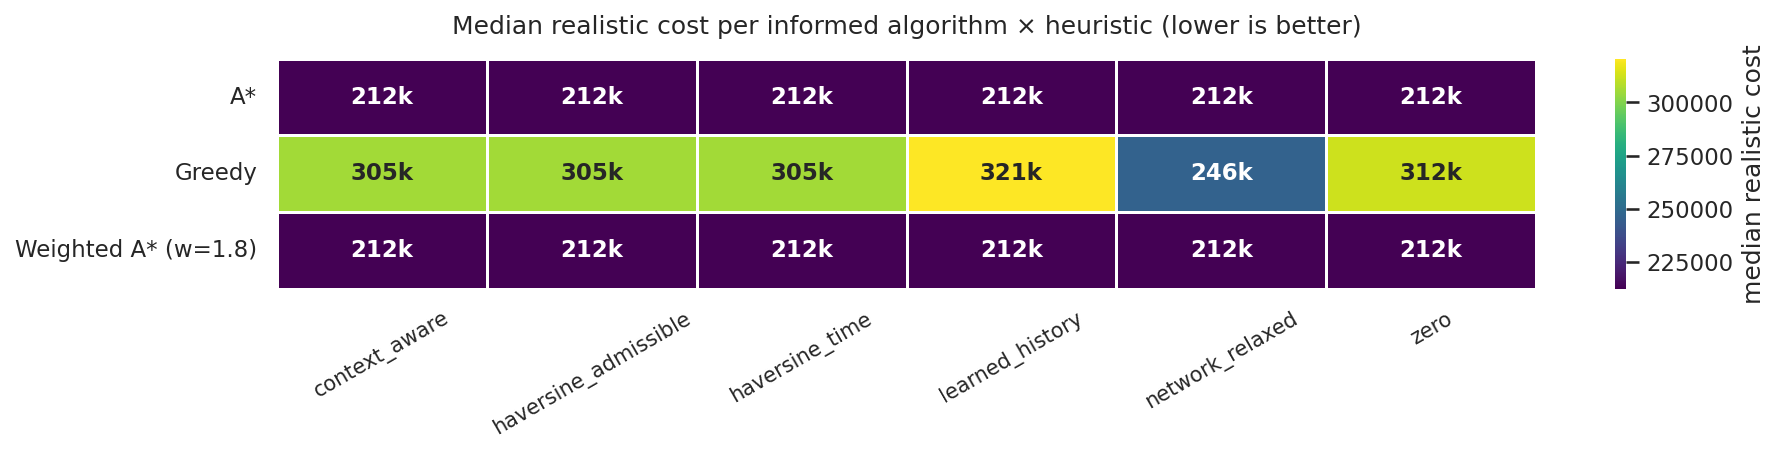
\includegraphics[width=0.86\textwidth]{figures/a1_heuristic_matrix.png}
  \caption{Nodes expanded for each (algorithm, heuristic) pair. The informed algorithms
  separate strongly from the uninformed ones; the heuristics separate only weakly from each
  other, because our admissible bound is loose.}
  \label{fig:a1heur}
\end{figure}

\section{Assignment 2: Fuel-Crisis Allocation as a Constraint Optimisation Problem}
\label{sec:a2}

\subsection{Problem Formulation}
A city is short of fuel. Stations hold limited reserves of petrol, diesel and octane; a
heterogeneous fleet of ambulances, buses, trucks, cars and motorbikes needs refuelling. If
every vehicle drives to its nearest station, the ambulances get stuck behind the motorbikes
and stations run dry of the wrong fuel.

We model it as a constraint \emph{optimisation} problem rather than a pure CSP, on the
principle that a system which returns nothing when the problem is infeasible is useless in a
crisis. Variables $X = \{x_1, \dots, x_N\}$, one per vehicle. The domain $D_i$ of $x_i$ is the
set of feasible (station, pump, time-slot) triples. Hard constraints: fuel-type compatibility;
reachability within the vehicle's remaining range; \emph{pump exclusivity} (no two vehicles at
the same pump in the same slot); station supply capacity per fuel type; and operating-hour
windows. The soft objective, to be minimised, is
\begin{equation}
J(S) = w_{\text{dist}} \cdot \text{distance} + w_{\text{wait}} \cdot \text{wait}
     + w_{\text{prio}} \cdot \text{priority penalty}
     + w_{\text{unassigned}} \cdot |\text{unassigned}|,
\end{equation}
with $w_{\text{unassigned}} = 100$. That last term is what turns the CSP into a COP: leaving
a vehicle unserved is expensive but legal, so the solver always returns its best partial
assignment.

\subsection{Methodology}
Five solvers: basic backtracking with no heuristics; backtracking + MRV; backtracking + LCV;
backtracking + forward checking + MRV + degree tie-break (with AC-3 as a one-shot preprocess);
and min-conflicts local search. Sizes $N \in \{10,20,30,40,50\}$, three seeds each, a 1.8\,s
wall-clock cap per run, and a 2{,}000-step budget for min-conflicts. We record nodes expanded,
backtracks, constraint checks, runtime, the final objective $J$, and the fraction of vehicles
left unassigned.

\subsection{Results and Discussion}
The main effect is the combinatorial blow-up. Basic backtracking expands
20.7 nodes at $N=10$ and 220{,}763 at $N=50$, roughly four orders of magnitude for a
five-fold increase in problem size, and at $N=50$ it never terminates on its own --- every
seed is pinned at the 1.8\,s cap with a success rate of 0. The composite solver
(FC + MRV + degree) expands 15{,}880 nodes at the same size, a 93\% reduction, and it is the
only complete solver that still finds a full assignment some of the time
(Table~\ref{tab:a2}).

\begin{table}[H]
\centering
\caption{Assignment 2 at the largest size, $N = 50$, mean over three seeds. Lower $J$ is better.}
\label{tab:a2}
\begin{tabular}{lrrrr}
\toprule
Solver & Nodes & Backtracks & Objective $J$ & Unassigned \\
\midrule
Basic backtracking & 220{,}763 & 220{,}728 & 3{,}542.0 & 29.3\% \\
Backtracking + MRV & 91{,}025 & 90{,}996 & 4{,}439.5 & 40.0\% \\
Backtracking + LCV & 18{,}891 & 18{,}863 & 4{,}188.9 & 43.3\% \\
FC + MRV + degree  & \textbf{15{,}880} & 15{,}833 & \textbf{1{,}718.4} & \textbf{6.7\%} \\
Min-conflicts      & 1{,}890$^{\dagger}$ & \textbf{0} & 1{,}927.8 & 8.0\% \\
\bottomrule
\end{tabular}

\vspace{0.4em}
{\footnotesize $^{\dagger}$ Repair steps, not tree nodes. Min-conflicts is not a tree search.}
\end{table}

Two results deserve comment because they are not what a naive reading of the textbook
predicts.

Min-conflicts performs exactly \textbf{zero} backtracks at every problem size. That is not a
bug and it is not an achievement --- it is definitional. Min-conflicts never builds a partial
assignment, so it has nothing to unwind. It starts complete and broken, and repairs. We flag
it because "backtracks" is on our metrics list and reporting a zero without explaining it
would look like a missing measurement.

The more awkward result is that plain MRV is \emph{worse} than basic backtracking on the
objective at $N=50$ (4{,}439 against 3{,}542) despite expanding four times fewer nodes. This
looked wrong until we looked at the unassigned column: MRV leaves 40\% of vehicles unplaced
against basic backtracking's 29\%. Since $w_{\text{unassigned}} = 100$ dominates $J$,
cross-solver comparisons of $J$ at large $N$ are really comparisons of how many vehicles got
dropped, and are confounded. Runtime at $N \geq 40$ is similarly not a measure of
time-to-solve; it is a measure of our time cap. We should have separated "quality of the
assignment made" from "how much of the problem was attempted", and we did not.

On the easy sizes the composite solver is essentially perfect: at $N=10$ and $N=20$ it expands
exactly $N$ nodes with 0 backtracks --- one node per variable, no wrong turns at all. Every
solver achieves 100\% success at $N \leq 20$; the phase transition to partial assignments
begins at $N = 30$.

\begin{figure}[H]
  \centering
  \begin{subfigure}{0.49\textwidth}
    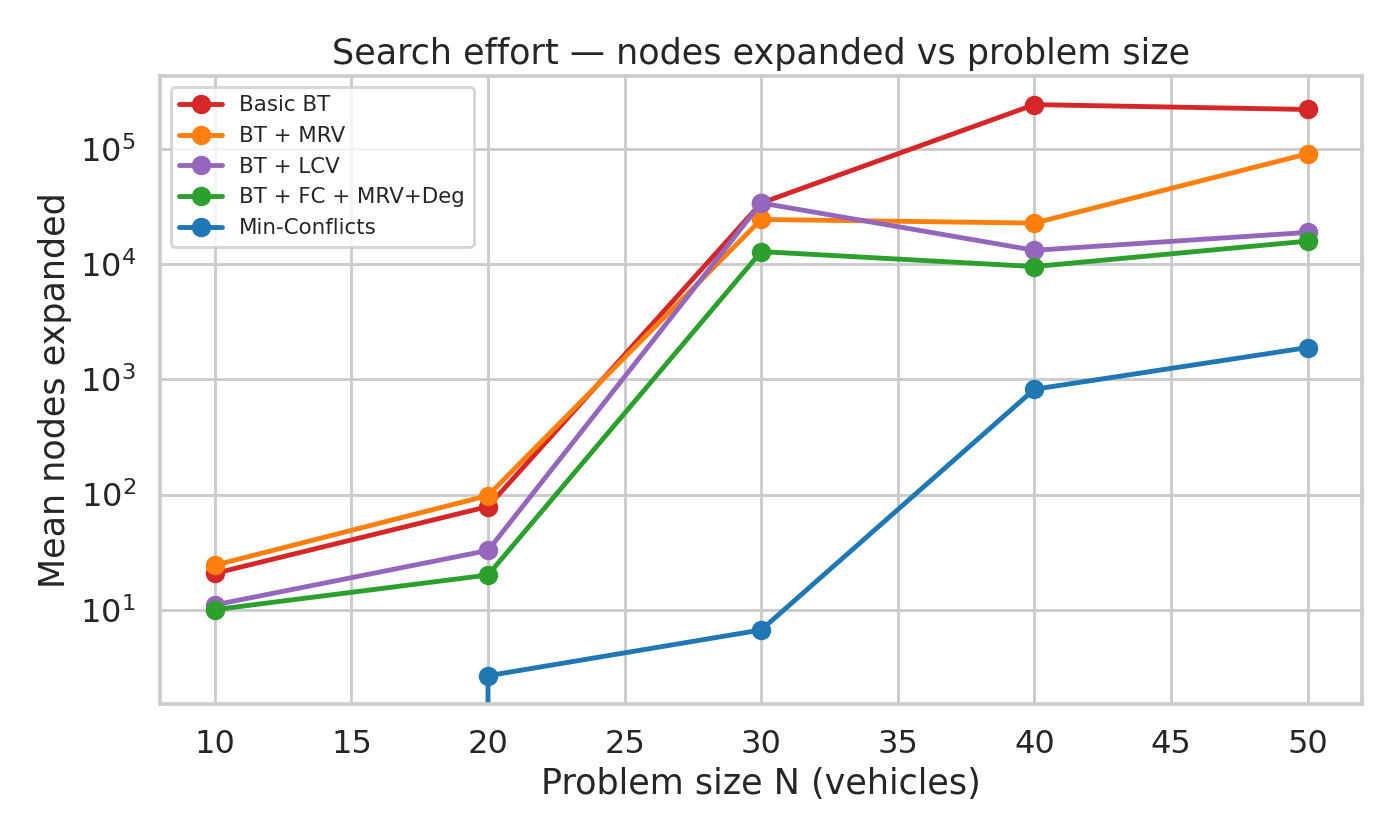
\includegraphics[width=\textwidth]{figures/a2_nodes_vs_n.png}
    \caption{Nodes expanded vs $N$ (log scale).}
  \end{subfigure}\hfill
  \begin{subfigure}{0.49\textwidth}
    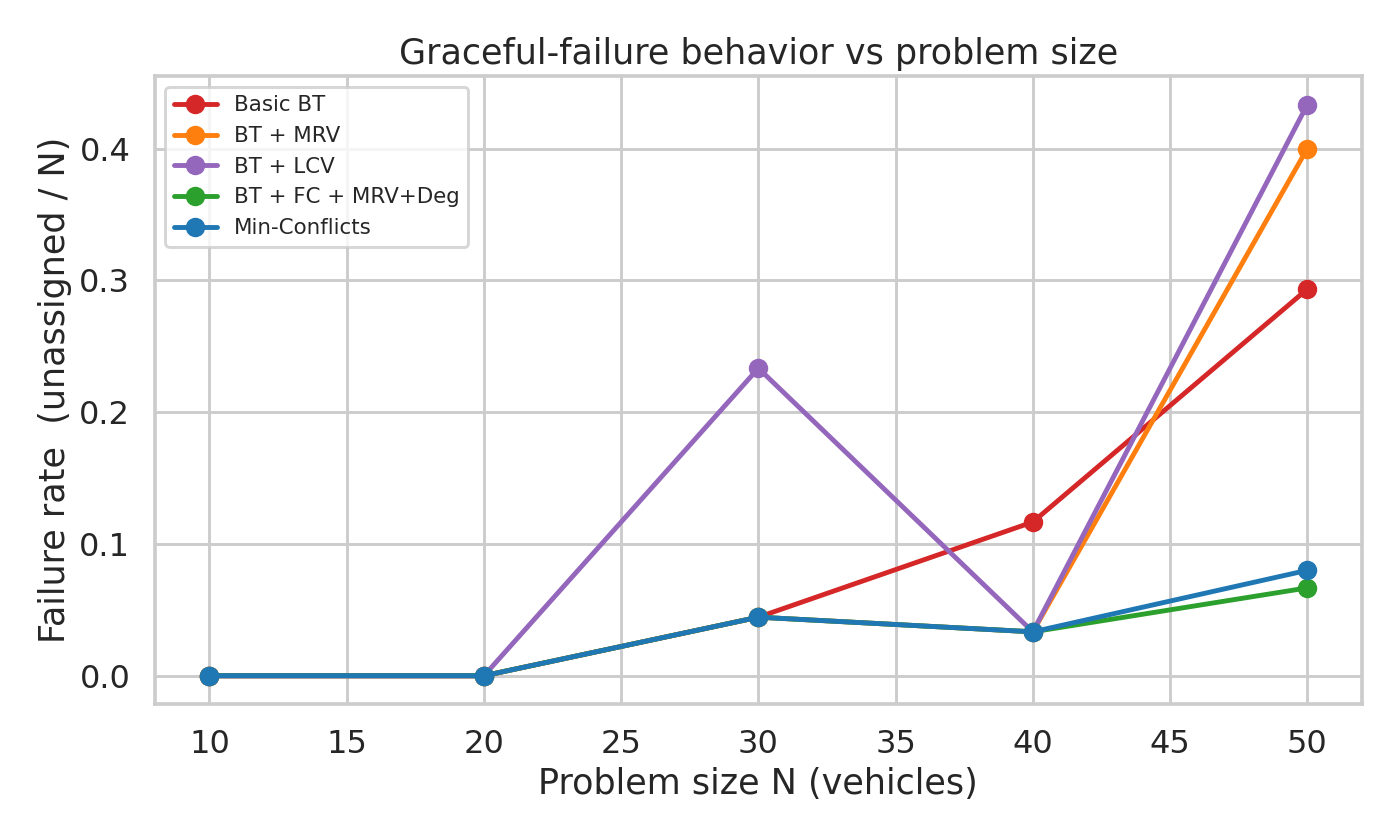
\includegraphics[width=\textwidth]{figures/a2_failure_rate_vs_n.png}
    \caption{Fraction of vehicles left unassigned.}
  \end{subfigure}
  \caption{Assignment 2. Propagation flattens the exponential; graceful degradation is what
  the COP formulation buys.}
  \label{fig:a2}
\end{figure}

\section{Assignment 3: Population-Based Search and Sequential Decision Making}
\label{sec:a3}

This assignment has two parts. Part~A requires a problem that a single weak agent cannot
solve but that a population of them can. Part~B requires a problem for Value Iteration and
Q-learning. We chose two separate problems rather than forcing one problem to serve both,
but they share a setting: a University of Dhaka residential hall. Part~A places its Wi-Fi;
Part~B runs its water pump.

% =====================================================================
\subsection{Part A --- Problem Formulation: Wi-Fi access-point placement}
The hall has a tight budget of $K$ access points for one floor. Rooms far from an AP, or
shadowed by a concrete partition, get an unusable signal. We choose the continuous positions
of the $K$ APs to maximise occupancy-weighted room coverage.

Decision variable: $\mathbf{x} = (\mathbf{a}_1, \dots, \mathbf{a}_K) \in \mathbb{R}^{2K}$, the
AP coordinates. Received signal at room $i$ from AP $j$ follows a log-distance indoor path-loss
model with discrete wall attenuation \citep{rappaport2002wireless}:
\begin{equation}
\mathrm{RSSI}_{ij} = P_{\text{tx}} - \bigl(L_0 + 10\,n \log_{10} d_{ij}\bigr) - \gamma\, c_{ij},
\end{equation}
where $c_{ij} \in \mathbb{Z}_{\geq 0}$ counts the concrete partitions the line of sight crosses.
Each room is served by its strongest AP, softened by a logistic so that signal \emph{margin}
is rewarded, and the objective is
\begin{equation}
\max_{\mathbf{x}} \quad F(\mathbf{x}) = \underbrace{100 \cdot \frac{\sum_i w_i\, \rho_i(\mathbf{x})}{\sum_i w_i}}_{\text{weighted coverage \%}}
\; - \; \lambda_{\text{sep}} \sum_{j<k} \bigl[\max(0,\, d_{\min} - \lVert \mathbf{a}_j - \mathbf{a}_k \rVert)\bigr]^2,
\end{equation}
subject to the APs lying inside the floor. The penalty term enforces a minimum separation
(co-channel interference).

Why this is not a gradient problem: $F$ contains a $\max_j$ (a kink), a logistic threshold,
and above all the \emph{integer} wall-crossing count $c_{ij}$, which makes $F$
piecewise-constant in $\mathbf{x}$. So $\nabla F = 0$ almost everywhere and is undefined on the
kinks. Exact enumeration is no better: the space is continuous, and discretising it throws
away the optimum, which is exactly what we demonstrate below.

Instance: a $60 \times 40$\,m hall block, 40 rooms with occupancy weights, 3 concrete
partitions, $K = 3$ APs (so a 6-dimensional search), $P_{\text{tx}} = 20$\,dBm,
$n = 3.3$, $\gamma = 8$\,dB, threshold $-66$\,dBm, $d_{\min} = 10$\,m.

\subsection{Part A --- Methodology}
We implemented the inertia-weight PSO of \citet{shi1998inertia}, which is the form on the
course slides:
\begin{align}
\mathbf{v} &\leftarrow w\,\mathbf{v} + c_1 r_1 (\mathbf{p}_{\text{best}} - \mathbf{x})
                                     + c_2 r_2 (\mathbf{g}_{\text{best}} - \mathbf{x}), \\
\mathbf{x} &\leftarrow \mathbf{x} + \mathbf{v}.
\end{align}
Each particle \emph{is} a complete candidate layout. The inertia $w$ decays linearly from 0.9
to 0.4, moving the swarm from exploration to exploitation; velocities are clamped to 20\% of
each axis range to stop the swarm exploding; positions are clamped to the floor with the
offending velocity component zeroed, which is constraint repair by an absorbing wall.
Swarm size 30, 100 iterations, $c_1 = c_2 = 1.49445$, 15 seeded runs.

The comparison is budget-matched, and we enforce it with an assertion at runtime rather than
trusting ourselves: one PSO run costs exactly $P(T+1) = 30 \times 101 = 3030$ fitness
evaluations, and Random Search is handed exactly 3030 samples. Grid Search lays a $5\times5$
lattice of candidate sites and evaluates all $\binom{25}{3} = 2300$ combinations, which fits
inside the budget with room to spare, so it is not truncated.

\subsection{Part A --- Results and Discussion}
\label{sec:a3a-results}
Under an identical 3{,}030-evaluation budget, PSO reaches a mean weighted coverage of 89.91\%
against 87.43\% for Random Search and 89.46\% for exhaustive Grid Search
(Table~\ref{tab:a3a}). The gain over random is 2.47 points, or 2.83\% in relative terms, and it
is significant by a one-sided Wilcoxon signed-rank test over the 15 paired seeds
($W = 120.0$, $p = 3.05 \times 10^{-5}$). PSO is also steadier: its run-to-run standard
deviation is 0.26 against random's 0.43, so its variance is about a third of random's.

\begin{table}[H]
\centering
\caption{Assignment 3A. Identical fitness-evaluation budget. Hard coverage is the percentage
of rooms actually above the usable-link threshold.}
\label{tab:a3a}
\begin{tabular}{lrrrrr}
\toprule
Method & Evals & Best & Mean & Std & Hard coverage \\
\midrule
PSO (ours)    & 3030 & \textbf{90.01} & \textbf{89.91} & 0.26 & \textbf{100.0\%} \\
Random Search & 3030 & 88.29 & 87.43 & 0.43 & 97.5\% \\
Grid Search   & 2300 & 89.46 & 89.46 & 0.00 & 100.0\% \\
\bottomrule
\end{tabular}
\end{table}

The Grid Search row is the one we care about, because it took two attempts to get right. In
our first instance the rooms sat on a perfect rectangular grid, and Grid Search \emph{beat}
PSO (89.19 against 88.41). That result was correct and it was our fault: if the demand points
are perfectly gridded, then grid-aligned AP positions are exactly where the optimum lives, and
we had handed the discrete method the answer. Real rooms are not perfectly gridded. We added
positional jitter ($\sigma = 1.5$\,m) so that the optimum sits \emph{off} any fixed lattice,
which is both more realistic and the whole reason to use a continuous optimiser. After that
change PSO wins. We report the earlier failure because it is the sharpest thing we learned in
this assignment: a discrete baseline can look strong for reasons that have nothing to do with
the algorithm.

\paragraph{Is the swarm actually doing anything?}
The assignment's real requirement is that individually weak agents solve collectively what
none can solve alone. That is a claim, so we tested it, with two ablations at the identical
3{,}030-evaluation budget (Figure~\ref{fig:a3collective}).

Shrink the swarm to a \emph{single} particle and give it all 3{,}030 evaluations to itself. With
one particle, $\mathbf{p}_{\text{best}}$ and $\mathbf{g}_{\text{best}}$ are the same point, the
social term vanishes identically, and PSO degenerates into one lone agent with momentum and a
memory. It scores 76.78, with a standard deviation of 6.66: not only much worse, but wildly
unreliable from run to run. This is the single weak agent the assignment asks us to beat.

The sharper experiment keeps all thirty particles and simply sets $c_2 = 0$. Same number of
agents, same budget, same everything; the particles still search and still remember their own
best. They just never tell each other anything. They score \textbf{87.30 $\pm$ 1.15} --- which
is statistically indistinguishable from Random Search's 87.43 $\pm$ 0.43.

That is the result we would defend the assignment on. Thirty independent searchers with no
communication are worth no more than throwing 3{,}030 darts. Restore one number --- the single
shared $\mathbf{g}_{\text{best}}$ --- and the same thirty agents, at the same cost, gain 2.61
points of fitness and connect every room in the hall instead of stranding one. The population is
not what helps. The communication is.

\begin{figure}[H]
  \centering
  \begin{subfigure}{0.52\textwidth}
    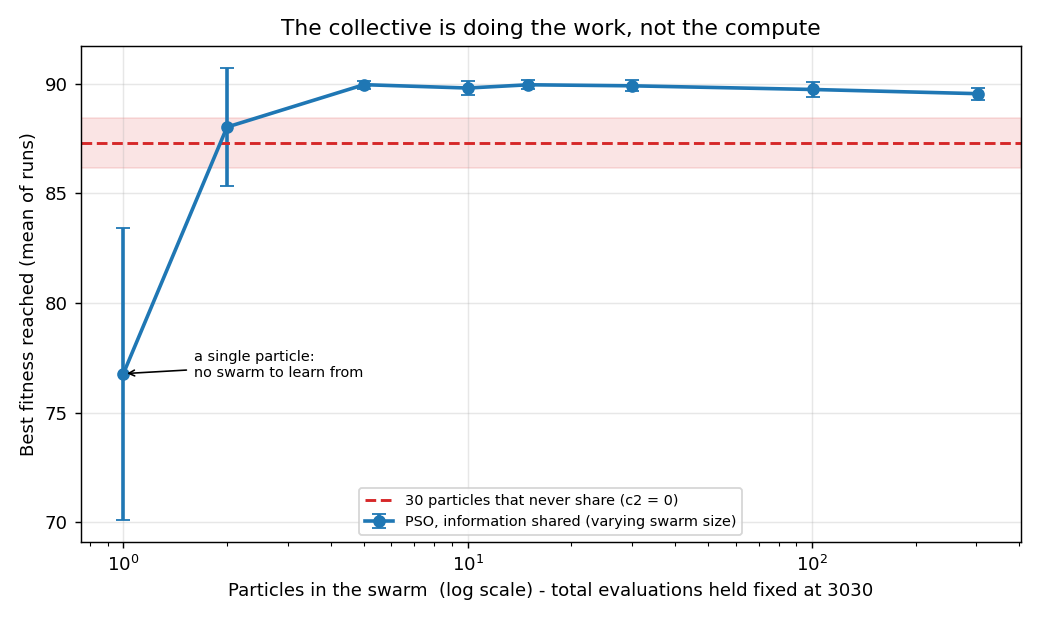
\includegraphics[width=\textwidth]{figures/a3_collective_behaviour.png}
    \caption{The ablation. Budget held fixed throughout.}
  \end{subfigure}\hfill
  \begin{subfigure}{0.46\textwidth}
    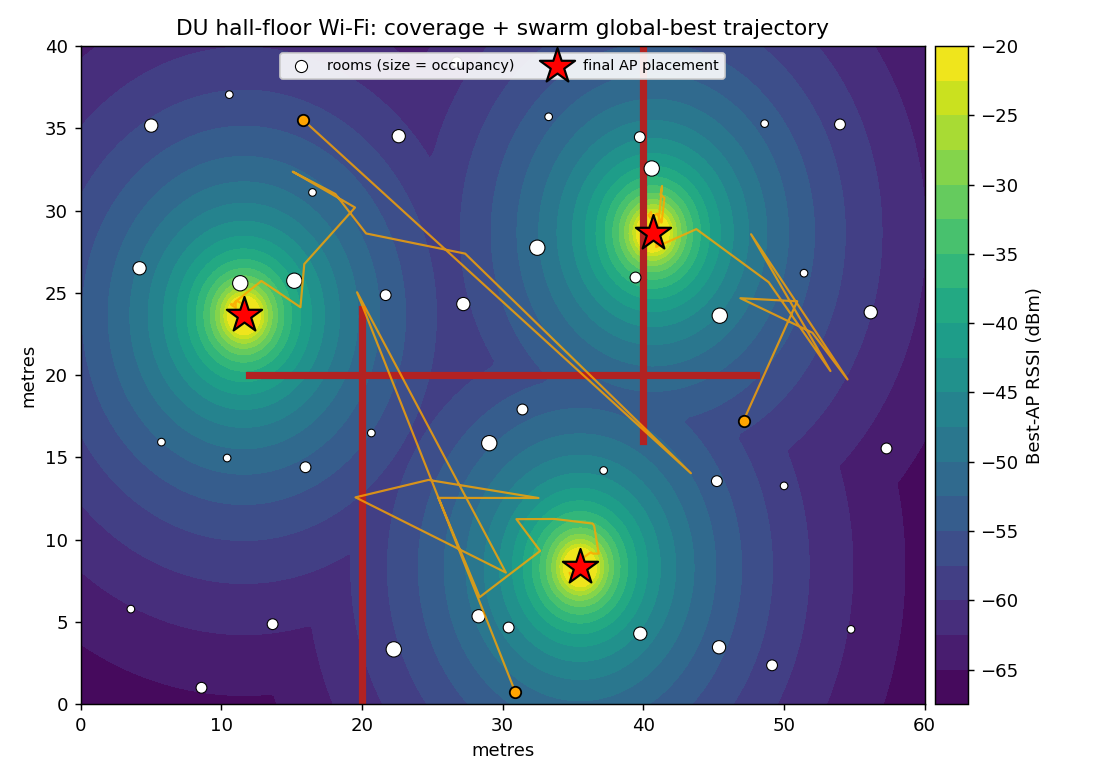
\includegraphics[width=\textwidth]{figures/a3_spatial_swarm.png}
    \caption{Coverage under the best layout, with the global-best trajectory.}
  \end{subfigure}
  \caption{Assignment 3A. Left: one particle scores 76.8; thirty silent particles score 87.3,
  no better than random; thirty communicating particles score 89.9. Right: the swarm's
  global-best APs migrating to their final positions (red stars) around the concrete
  partitions.}
  \label{fig:a3collective}
\end{figure}

The swarm-size curve also shows the expected U-shape. At a fixed budget, too few particles
means no information to share; too many means too few iterations to use it. Five to fifteen
particles is the sweet spot here (89.95), and 303 particles --- which leaves only 10 iterations
--- falls back to 89.55.

\paragraph{How much should they talk?}
Having established that communication matters, the obvious next question is whether \emph{more}
of it is better, and here the literature makes a specific prediction.
\citet{kennedy2002population} compare seventy swarm topologies and conclude that "greater
connectivity speeds up convergence, though it does not tend to improve the population's ability
to discover global optima" --- their fully-connected swarm reached its criterion in a median of
404.8 iterations but only 85\% of the time, against a ring's 755.5 iterations and 94\%. They
also warn that inhibiting communication too far leaves particles "wandering cluelessly", which
is precisely our $c_2 = 0$ result.

We implemented a ring topology, in which each particle hears only its immediate neighbours
around a circle, so a good discovery has to walk around the ring one hop per iteration instead
of being broadcast instantly. Over 30 paired seeds at the same budget:

\begin{table}[H]
\centering
\caption{Communication topology. Same 30 particles, same 3{,}030 evaluations. The only thing
that changes is who can hear whom.}
\label{tab:a3topo}
\begin{tabular}{lrrr}
\toprule
Topology & Mean & Std & Stagnates at \\
\midrule
No communication ($c_2 = 0$) & 87.30 & 1.151 & iter 53 \\
Fully connected (\emph{gbest}) & 89.83 & 0.317 & iter \textbf{83} \\
Ring, $k = 1$ & 89.96 & \textbf{0.129} & iter \textbf{100} \\
\bottomrule
\end{tabular}
\end{table}

The result is not the one we first wrote down. Our initial draft reported that the ring was
simply better; a unit test asserting that failed on a different set of seeds, which was the
correct outcome. Tested properly, the mean difference is \textbf{not significant} (Wilcoxon,
$p = 0.92$) while the variance difference \textbf{is}, by a factor of six ($F$-test,
$p = 6 \times 10^{-6}$). The fully-connected swarm quits at iteration 83; the ring is still
improving when the budget runs out.

So the ring does not find a \emph{better} answer. It finds a \emph{consistent} one. That is
exactly what \citet{kennedy2002population} predict, and it is worth being careful about what
they do \emph{not} say: they rank the ring 64th of the 70 topologies they tried and recommend a
von Neumann lattice instead. We have not tried that, and it is the obvious next experiment.

% =====================================================================
\subsection{Part B --- Problem Formulation: the hall water tank under load-shedding}
The same hall keeps its water in an overhead tank fed by an electric pump. Three things make
this a decision problem and not a plumbing one. The grid fails, and it fails hardest in the
evening, when the hall wants water. Evening outages are also long: once the power goes it tends
to stay gone. And the hall owns a diesel generator that can drive the pump through an outage,
but it buys a fixed ration of diesel each morning --- burn it at 7am on a hunch and there is
none left at 9pm.

Formally, an infinite-horizon discounted MDP. State $s = (L, t, g, F)$ with tank level
$L \in \{0..10\}$ (units of 100\,L), hour $t \in \{0..23\}$ (wrapping; this is a continuing
task), grid up $g \in \{0,1\}$, and diesel remaining $F \in \{0,1,2\}$. That is
$11 \times 24 \times 2 \times 3 = 1584$ states. Actions are $\{$idle, pump on grid, pump on
diesel$\}$, restricted by a state-dependent availability mask: pumping on grid is not offered
during an outage (the switch does nothing) and diesel is not offered when the drum is empty.

Demand is a truncated Poisson whose mean depends on the hour, with peaks at 06:00--09:00 and
18:00--22:00. The grid is a two-state Markov chain whose failure and restore probabilities
depend on the hour; in the evening, failure probability is 0.35 and restore is only 0.15, so an
evening outage lasts about 6.7 hours in expectation. The reward is
\begin{equation}
r = -\bigl(\text{pump cost} + c_{\text{overflow}}\cdot\text{spill}
    + c_{\text{shortage}}\cdot U\bigr),
\end{equation}
with $c_{\text{shortage}} = 20$ per unit of water students wanted and did not get, against a
grid pump-hour cost of 1 and a diesel pump-hour cost of 6. We use $\gamma = 0.99$: at one hour
per step that is an effective horizon of 100 hours, comfortably longer than the 24-hour cycle
the whole problem turns on.

One subtlety that matters. The realised shortage $U$ depends on the realised demand $D$, and
$D$ is \emph{not} recoverable from $s'$ --- once the tank hits zero you cannot tell how much
demand went unmet. So $r$ is not a function of $(s,a,s')$. This is fine, and it is the standard
disturbance form of an MDP: $r = r(s,a,w)$ with $w = (D, g')$. Value Iteration only ever needs
the expected reward $R(s,a) = \mathbb{E}_w[r]$, which is what we tabulate, and the Bellman
operator is still a $\gamma$-contraction. Q-learning consumes the \emph{realised} $r$. It has to:
if we fed it $\mathbb{E}[U]$ we would have leaked the demand distribution into the "model-free"
agent, and the entire distinction the assignment is about would collapse.

\subsection{Part B --- Methodology}
We built the MDP with two faces that must never disagree. \code{build\_model()} returns the
explicit sparse $P(s'\mid s,a)$ and $R(s,a)$ that Value Iteration consumes. \code{step()} returns
one sampled $(s', r)$ and no probability ever leaves it; that is the only thing Q-learning is
allowed to call. A unit test Monte-Carlo-estimates $P$ and $R$ back out of \code{step()} over
8{,}000 samples per state-action pair and asserts they match the table within sampling error.
Without that gate, the classic silent failure is that the two faces disagree about, say, whether
the pump acts before or after demand, Q-learning converges to a different optimum, and you spend
a week blaming the learning rate.

\textbf{Value Iteration} sweeps $V_{k+1}(s) = \max_{a \in A(s)} [R(s,a) + \gamma \sum_{s'}
P(s'|s,a) V_k(s')]$ to a residual of $10^{-9}$.

\textbf{Q-learning} runs $\varepsilon$-greedy on the simulator with the update
$Q(s,a) \leftarrow Q(s,a) + \alpha [r + \gamma \max_{a'} Q(s',a') - Q(s,a)]$. We use exploring
starts (a uniformly random state each episode), because without them large parts of the state
space are never visited under a decent policy and the argmax there is meaningless. The learning
rate is $\alpha_n = 1/(1+n(s,a))^{0.7}$, which satisfies Robbins--Monro
\citep{evendar2003rates}. Episodes are 24 hours, but the task is continuing, so we bootstrap
normally at the cut and never zero the terminal value.

Every policy in this section --- Value Iteration's, Q-learning's, and the baselines' --- is scored
the same way: by \emph{exactly} solving the linear system $(I - \gamma P_\pi)V^\pi = R_\pi$ under
the \emph{true} model. This removes Monte-Carlo evaluation noise from the comparison entirely.
Policies are ranked by their exact expected return, not by which one drew a luckier rollout.

Baselines. The \emph{myopic} policy is Value Iteration with $\gamma = 0$: the formally correct
greedy rule, not a strawman. The \emph{caretaker} policy is a two-threshold reactive rule (pump
on grid below level $T_g$, run diesel below level $T_d$) with the \emph{same action set} as the
optimal policy, and we grid-search both thresholds and report its best version. Beating a
crippled baseline would prove nothing.

We also added a baseline that could sink our whole thesis, which we will come to.

\subsection{Part B --- Results and Discussion}

\paragraph{Value Iteration behaves exactly as the theory says.}
It converges in 2{,}273 sweeps (0.23\,s), and the Bellman residual decays at an empirical rate
of \textbf{0.9900} --- which is $\gamma$ to four decimal places, as the contraction mapping
theorem requires (Figure~\ref{fig:a3vi}). Independently, $V^*$ from iterating the optimality
operator agrees with $V^{\pi^*}$ from directly solving the linear system to
$1.8 \times 10^{-8}$. Two different routes, one answer.

\paragraph{The problem genuinely needs lookahead.}
This had to be checked, because if a greedy rule were nearly optimal the assignment would be
vacuous. It is not. The myopic $\gamma = 0$ policy loses \textbf{121\%}, and even the best tuned
reactive threshold rule --- which has the generator, and whose thresholds we optimised for it ---
still loses \textbf{14.5\%} (Table~\ref{tab:a3b}).

\begin{table}[H]
\centering
\caption{Assignment 3B. Exact expected return under the true model; rollout statistics over
1{,}000 simulated days.}
\label{tab:a3b}
\begin{tabular}{lrrrr}
\toprule
Policy & Exact $V$ & Regret & Cost/day & Shortage units/day \\
\midrule
Value Iteration (optimal)      & \textbf{-163.6} & \textbf{0\%} & \textbf{32.8} & \textbf{0.78} \\
Tuned caretaker rule           & -187.4 & 14.5\%  & 36.9 & 0.94 \\
Myopic greedy ($\gamma = 0$)   & -361.0 & 120.6\% & 78.1 & 3.08 \\
Random (legal actions)         & -697.5 & 326.2\% & 166.3 & 6.85 \\
Always idle                    & -2507.8 & 1432.5\% & 527.7 & 26.38 \\
\bottomrule
\end{tabular}
\end{table}

We can point at the anticipation directly. At 14:00 with a 4/10 tank and the grid up, pumping
costs 0.97 \emph{more} than idling this hour, and the optimal policy pumps anyway, because the
action is worth $+4.69$ overall. Of that advantage, $+5.66$ comes purely from the future. The
agent is paying now for water it will need after the lights go out. Figure~\ref{fig:a3policy}
shows this structurally: the region where the optimal policy burns diesel expands sharply once
the evening window opens.

\paragraph{The main experiment, and the answer we did not want.}
The obvious story to tell is "Dhaka's published load-shedding schedule is optimistic, so a
planner using it will be wrong, so use model-free Q-learning instead." We set out to
demonstrate that, and the data refused.

We gave Value Iteration a \emph{deliberately wrong} model, scaling the believed grid-failure
probability by a factor and then scoring the resulting policy in the real hall
(Figure~\ref{fig:a3mismatch}). Value Iteration turned out to be far less sensitive to this than we expected. Believing outages are
twice as rare as they are costs only 1.5\% regret. Four times as rare costs 2.7\%. You have to
tell the planner the grid \emph{never} fails before its regret (21.4\%) exceeds Q-learning's.

Meanwhile Q-learning, after 720{,}000 environment steps (that is 82 simulated \emph{years} of
hourly hall operation), sits at \textbf{15.1\% $\pm$ 2.4} regret, with 100\% coverage of the
legal state-action space. It is converging, but slowly, and $\gamma = 0.99$ is part of why: a
long effective horizon and a high-variance reward (a shortage costs 20 in a single hour) is a
punishing combination for a tabular method.

Then we added the arm that could falsify us. Take the \emph{same} transitions Q-learning
consumed, count them into a maximum-likelihood estimate $\hat{P}(s'|s,a) = N(s,a,s')/N(s,a)$,
and run Value Iteration on that. Same samples, two different ways of spending them. This
\emph{certainty-equivalence} planner reaches \textbf{1.4\% $\pm$ 0.2} regret, ten times better
than the Q-learner trained on identical data.

But it does \emph{not} beat every prior. A planner who is only mildly wrong --- believing
outages are 1.25$\times$ or 0.75$\times$ their true rate --- scores 0.11\% and 0.24\%, which is
better than the model we learned from 720{,}000 samples. Certainty-equivalence only overtakes
the prior once the prior is \emph{badly} wrong (at or beyond a factor of two in either
direction). We had written the opposite in an earlier draft, and the table we printed directly
underneath it said so; the corrected statement is the more interesting one.

Ranking everything by regret makes the picture plain:

\begin{table}[H]
\centering
\caption{Everything, ranked. Regret against the exact optimum, under the true model.}
\label{tab:a3rank}
\begin{tabular}{llr}
\toprule
& What it knows & Regret \\
\midrule
Value Iteration, correct model      & the exact $P$                    & 0\% \\
Value Iteration, mildly wrong model & $P$ off by $1.25\times$          & 0.1\% \\
                                    & $P$ off by $0.75\times$          & 0.2\% \\
Certainty-equivalence VI            & $\hat{P}$ from 720k samples      & 1.4\% \\
Value Iteration, badly wrong model  & $P$ off by $4\times$             & 2.7\% \\
                                    & $P$ off by $10\times$            & 6.7\% \\
Tuned caretaker threshold rule      & nothing; two tuned numbers       & 14.5\% \\
Q-learning                          & 720k samples, no model           & 15.1\% \\
Value Iteration, no outage model    & believes the grid never fails    & 21.4\% \\
Myopic greedy ($\gamma = 0$)        & the model, but no future         & 120.6\% \\
\bottomrule
\end{tabular}
\end{table}

\paragraph{Why does the learned model beat the learner by ten times?}
We had this measurement before we had an explanation for it, and the explanation turns out to be
a proved separation rather than a quirk of our hall. \citet{agarwal2020modelbased} show that the
plug-in (certainty-equivalence) estimator --- build $\hat{P}$ from samples, plan optimally in the
empirical MDP --- is \emph{minimax optimal}, attaining
$\tilde{\Theta}\bigl(|S||A| / ((1-\gamma)^3\varepsilon^2)\bigr)$.
\citet{li2024qlearning} settle vanilla synchronous Q-learning at
$\tilde{\Theta}\bigl(|S||A| / ((1-\gamma)^4\varepsilon^2)\bigr)$ and state that this "unveils the
strict sub-optimality of Q-learning when $|A| \geq 2$".

The gap is a full factor of $1/(1-\gamma)$ in the effective horizon. We chose $\gamma = 0.99$, so
that factor is \textbf{100}. The theory predicts our Q-learner should be about two orders of
magnitude behind in sample efficiency purely because of the discount, and a ten-fold regret gap
at a fixed 720{,}000 samples is what that looks like from the inside.

The mechanism is not mysterious once stated: a Q-learning update spends a transition on one cell
of the table and then discards it, whereas a learned model \emph{stores} it and every subsequent
Bellman backup re-reads it, so one sample propagates across the whole state space instead of into
the single cell where it landed.

One caveat we will not drop, because it is the difference between a true claim and a sloppy one:
this separation is against \emph{vanilla tabular} Q-learning, not against model-free RL in
general --- variance-reduced Q-learning variants do reach the optimal rate. (We also note that we
nearly cited \citet{azar2013minimax} for this. It does not support the claim: its lower bound is
information-theoretic and binds model-free methods equally.)

So the honest conclusion inverts the one we went looking for:

\begin{itemize}
  \item A roughly-right model is worth more than 82 simulated years of experience. That is the
        result we did not expect and it is the one we would lead with.
  \item Value Iteration degrades gracefully. A planner with a fourfold error in its outage
        estimate (2.7\%) still comfortably beats a Q-learner given 720{,}000 steps (15.1\%).
  \item Our Q-learner also loses to the tuned two-parameter threshold rule (14.5\%), which does
        no learning at all. We would rather state that than have it extracted from us.
  \item Therefore the case for model-free learning here is \emph{not} "the model might be
        wrong" --- it can be quite wrong and still win. It is narrower and it is real:
        model-free is what you reach for when you cannot write down the transition structure at
        all. Ours has 1{,}584 states and we could write it down, which makes this an honest
        advertisement for Value Iteration and a poor one for Q-learning. Knowing why is the
        point.
\end{itemize}

\begin{figure}[H]
  \centering
  \begin{subfigure}{0.49\textwidth}
    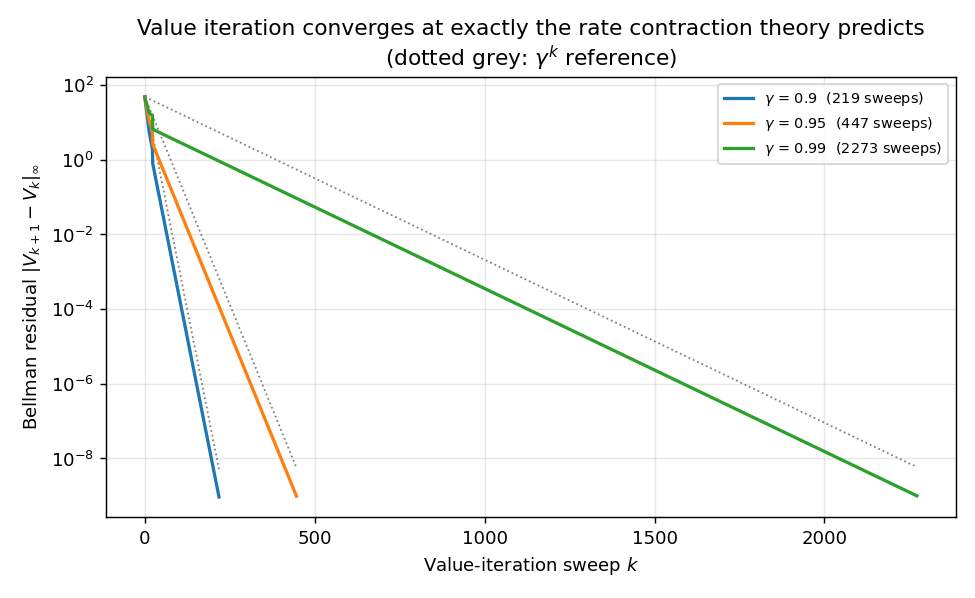
\includegraphics[width=\textwidth]{figures/a3_rl_vi_convergence.png}
    \caption{Contraction at rate $\gamma$, as predicted.}
    \label{fig:a3vi}
  \end{subfigure}\hfill
  \begin{subfigure}{0.49\textwidth}
    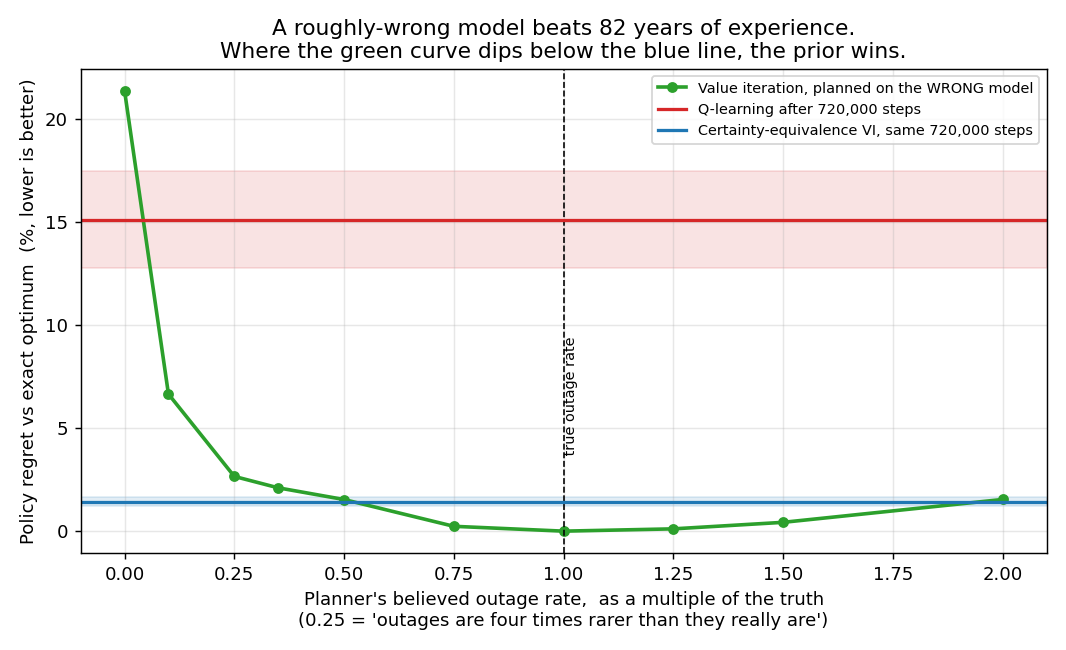
\includegraphics[width=\textwidth]{figures/a3_rl_model_mismatch.png}
    \caption{How wrong can a prior model be?}
    \label{fig:a3mismatch}
  \end{subfigure}
  \caption{Assignment 3B. Right: the green curve is Value Iteration planned on a wrong model
  and scored in the real hall. It stays below Q-learning's red band until the planner believes
  the grid essentially never fails. The blue line is a model estimated from Q-learning's own
  samples.}
\end{figure}

\begin{figure}[H]
  \centering
  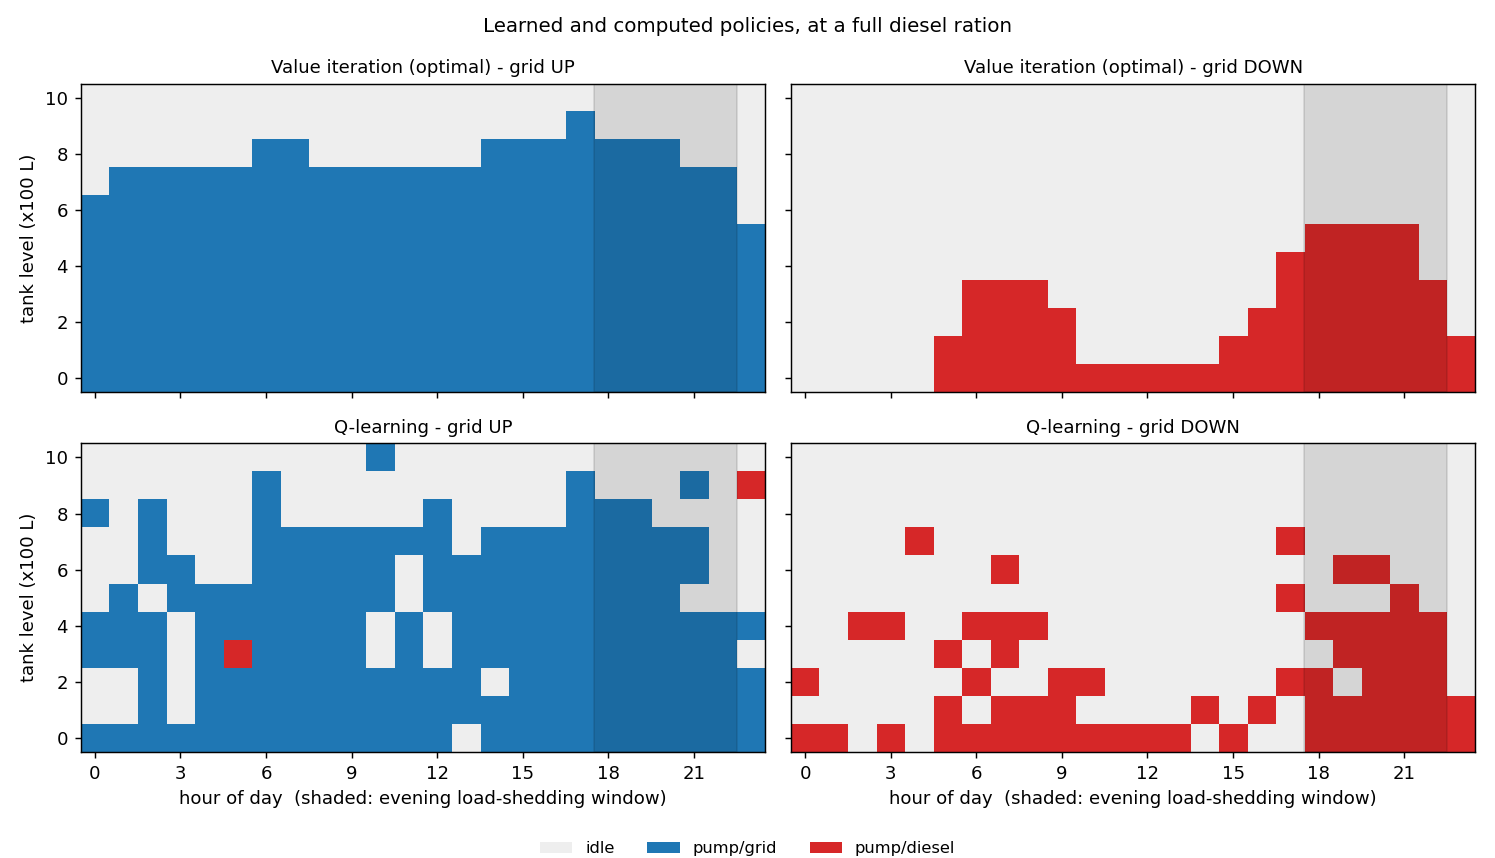
\includegraphics[width=0.92\textwidth]{figures/a3_rl_policy_maps.png}
  \caption{Policies at a full diesel ration. Value Iteration (top) is clean and shows the
  diesel region expanding into the shaded evening outage window --- that is anticipation. Q-learning
  (bottom) recovers the same structure but speckled, which is what an under-trained tabular
  learner looks like. It picks an optimal action in 86.6\% of states.}
  \label{fig:a3policy}
\end{figure}

\paragraph{Hyperparameters.}
Table~\ref{tab:a3hp} sweeps Q-learning's knobs at 8{,}000 episodes and 3 seeds. Two findings and
one non-finding.

The two that matter are both large. Turning off exploring starts triples regret (76.7\% against
25.1\%): without random resets the agent simply never sees much of the state space. And the
learning-rate schedule behaves exactly as \citet{evendar2003rates} says it must --- the
Robbins--Monro polynomial rate reaches 25.1\% while a constant $\alpha = 0.1$ stalls at 50.4\%
and $\alpha = 0.5$ at 57.9\%. A constant step size converges only to a neighbourhood of $Q^*$,
and here you can watch it happen.

The non-finding is exploration. Varying the $\varepsilon$ floor from 0.01 to 0.05 to 0.20 gives
30.6\%, 25.1\% and 27.5\%, non-monotonic and inside the seed noise. We tried values from one end
of the sensible range to the other and it did not much matter, so that is what we report.

Two results surprised us and we do not want to bury them. Pessimistic initialisation
($Q_0 = -200$) does slightly \emph{better} than the zero initialisation (21.1\% against 25.1\%),
which is the opposite of what we predicted --- we had expected zero-init to be helpfully
optimistic, since every reward in this MDP is non-positive. The likely explanation is scale:
$V^*$ is around $-164$, so $Q_0 = -200$ starts far closer to the truth than $Q_0 = 0$ does, and
that head start outweighs the lost optimism. Similarly, training with $\gamma = 0.9$ produces a
policy that scores \emph{better} (19.5\%) than training with $\gamma = 0.99$ (25.1\%) even when
both are judged under the $\gamma = 0.99$ criterion. A shorter training horizon means lower
variance and faster credit assignment, and here that is worth more than matching the evaluation
discount. We chose $\gamma = 0.99$ on principle, and the data says the principle cost us
something.

\begin{table}[H]
\centering
\caption{Assignment 3B hyperparameter sweep. Mean regret over 3 seeds, 8{,}000 episodes each.}
\label{tab:a3hp}
\begin{tabular}{llr}
\toprule
Group & Setting & Regret \% \\
\midrule
Learning rate  & polynomial $1/(1+n)^{0.7}$ & 25.1 $\pm$ 2.1 \\
               & polynomial $1/(1+n)^{0.5}$ & 28.2 $\pm$ 5.9 \\
               & constant $\alpha = 0.10$   & 50.4 $\pm$ 2.9 \\
               & constant $\alpha = 0.50$   & 57.9 $\pm$ 3.8 \\
\midrule
Exploration    & $\varepsilon$ floor 0.01   & 30.6 $\pm$ 5.7 \\
               & $\varepsilon$ floor 0.05   & 25.1 $\pm$ 2.1 \\
               & $\varepsilon$ floor 0.20   & 27.5 $\pm$ 5.3 \\
               & \textbf{exploring starts off} & \textbf{76.7 $\pm$ 7.0} \\
\midrule
Initialisation & $Q_0 = 0$ (optimistic here) & 25.1 $\pm$ 2.1 \\
               & $Q_0 = -200$ (pessimistic)  & 21.1 $\pm$ 1.3 \\
\midrule
Discount       & $\gamma = 0.90$ & 19.5 $\pm$ 1.4 \\
               & $\gamma = 0.95$ & 25.8 $\pm$ 1.4 \\
               & $\gamma = 0.99$ & 25.1 $\pm$ 2.1 \\
\bottomrule
\end{tabular}
\end{table}

\paragraph{Limitations we know about.}
Our grid model is a two-state Markov chain, which makes outage durations geometric: an outage
that has already run four hours is exactly as likely to end as one that just started. Real
Dhaka load-shedding is largely \emph{scheduled} and rotational, so durations are far more
predictable than that. Modelling the true environment as semi-Markov while the planner keeps
the two-state chain would be \emph{structural} mis-specification, which cannot be fixed by
re-estimating a parameter, and we suspect that is the regime where model-free learning would
finally have a real story to tell. We did not do it, and we think it is the single most
interesting thing left on the table.

We also chose the discounted criterion rather than average reward. For a continuing operations
problem, average cost per hour is arguably the more natural objective, and the discounted-optimal
policy is not guaranteed to be gain-optimal. We report discounted return consistently everywhere
and never draw a discounted $V^*$ line on an average-cost axis, but the choice is a choice.

\section{Conclusions}
\label{sec:conc}
Four things we take away.

An admissible heuristic is easy to construct and hard to make tight. In Assignment~1 our heuristic is
provably admissible and buys only an 11\% reduction in nodes expanded, because on a
twelve-factor multiplicative cost model the "best possible cost per metre" bound is extremely
loose. Greedy Best-First, which abandons the guarantee entirely, is 79 times cheaper and 38\%
worse. The guarantee and its price are both real.

Propagation is what makes constraint search tractable. Forward checking with MRV cut nodes
expanded by 93\% at $N=50$. But we also learned
that our objective confounds solution quality with coverage at large $N$, which made plain MRV
look worse than no heuristic at all. Designing the metric is part of designing the experiment,
and we got that wrong the first time.

The swarm's advantage is the communication, not the population. This is the result we are most
confident in, because we tried hard to destroy it. Thirty particles that do not share are worth
no more than random sampling; the same thirty sharing a single number gain 2.47 points and
connect every room. That is the assignment's thesis, and it survived our attempt to break it.

And the most useful thing we learned is a negative result. We expected to show that model-free
Q-learning beats a planner working from Dhaka's optimistic load-shedding schedule. It does not.
A planner whose outage estimate is wrong by a factor of four still beats a Q-learner given
720,000 steps, and a planner who is only mildly wrong beats even the model we estimated from
those same samples. The real argument for model-free control is not that models are often wrong,
because they can be quite wrong and still win. It is that sometimes you cannot write one down at
all. Our problem was small enough to write down, so it is an honest advertisement for Value
Iteration and a poor one for Q-learning. We would rather report that than the story we went
looking for.

Future work, in the order we would actually do it: make the load-shedding process semi-Markov so
that the planner's state is not even Markov with respect to reality; tighten the Assignment~1
heuristic; and separate quality from coverage in the Assignment~2 objective.

\bibliographystyle{plainnat}
\bibliography{references}

\end{document}
